% Beamer Presentation
% LaTeX Template
% Version 1.0 (10/11/12)
%
% This template has been downloaded from:
% http://www.LaTeXTemplates.com
%
% License:
% CC BY-NC-SA 3.0 (http://creativecommons.org/licenses/by-nc-sa/3.0/)
%
%%%%%%%%%%%%%%%%%%%%%%%%%%%%%%%%%%%%%%%%%

%----------------------------------------------------------------------------------------
%	PACKAGES AND THEMES
%----------------------------------------------------------------------------------------

\documentclass{beamer}

\mode<presentation> {

% The Beamer class comes with a number of default slide themes
% which change the colors and layouts of slides. Below this is a list
% of all the themes, uncomment each in turn to see what they look like.

%\usetheme{default}
%\usetheme{AnnArbor}
%\usetheme{Antibes}
%\usetheme{Bergen}
%\usetheme{Berkeley}
%\usetheme{Berlin}
%\usetheme{Boadilla}
%\usetheme{CambridgeUS}
%\usetheme{Copenhagen}
%\usetheme{Darmstadt}
%\usetheme{Dresden}
%\usetheme{Frankfurt}
%\usetheme{Goettingen}
%\usetheme{Hannover}
%\usetheme{Ilmenau}
%\usetheme{JuanLesPins}
%\usetheme{Luebeck}
\usetheme{Madrid}
%\usetheme{Malmoe}
%\usetheme{Marburg}
%\usetheme{Montpellier}
%\usetheme{PaloAlto}
%\usetheme{Pittsburgh}
%\usetheme{Rochester}
%\usetheme{Singapore}
%\usetheme{Szeged}
%\usetheme{Warsaw}

% As well as themes, the Beamer class has a number of color themes
% for any slide theme. Uncomment each of these in turn to see how it
% changes the colors of your current slide theme.

%\usecolortheme{albatross}
%\usecolortheme{beaver}
%\usecolortheme{beetle}
%\usecolortheme{crane}
%\usecolortheme{dolphin}
%\usecolortheme{dove}
%\usecolortheme{fly}
%\usecolortheme{lily}
%\usecolortheme{orchid}
%\usecolortheme{rose}
%\usecolortheme{seagull}
%\usecolortheme{seahorse}
%\usecolortheme{whale}
%\usecolortheme{wolverine}

%\setbeamertemplate{footline} % To remove the footer line in all slides uncomment this line
%\setbeamertemplate{footline}[page number] % To replace the footer line in all slides with a simple slide count uncomment this line

%\setbeamertemplate{navigation symbols}{} % To remove the navigation symbols from the bottom of all slides uncomment this line
}

\usepackage{graphicx} % Allows including images
\usepackage{booktabs} % Allows the use of \toprule, \midrule and \bottomrule in tables

%----------------------------------------------------------------------------------------
%	TITLE PAGE
%----------------------------------------------------------------------------------------

\title[Short title]{Full Title of the Talk} % The short title appears at the bottom of every slide, the full title is only on the title page

\author{John Smith} % Your name
\institute[UCLA] % Your institution as it will appear on the bottom of every slide, may be shorthand to save space
{
University of California \\ % Your institution for the title page
\medskip
\textit{john@smith.com} % Your email address
}
\date{\today} % Date, can be changed to a custom date

\begin{document}

\begin{frame}
\titlepage % Print the title page as the first slide
\end{frame}

\begin{frame}
\frametitle{Overview} % Table of contents slide, comment this block out to remove it
\tableofcontents % Throughout your presentation, if you choose to use \section{} and \subsection{} commands, these will automatically be printed on this slide as an overview of your presentation
\end{frame}

%----------------------------------------------------------------------------------------
%	PRESENTATION SLIDES
%----------------------------------------------------------------------------------------

%------------------------------------------------
\section{First Section} % Sections can be created in order to organize your presentation into discrete blocks, all sections and subsections are automatically printed in the table of contents as an overview of the talk
%------------------------------------------------

\subsection{Subsection Example} % A subsection can be created just before a set of slides with a common theme to further break down your presentation into chunks

\begin{frame}
\frametitle{ Applications for Identity-Based Encryption}
\subsection{ Revocation of Public Keys}
\begin{enumerate}
\item  Revocation of Public Keys\\
Public key certificates are valid, an IBE system key expiration can be done by
having Alice encrypt e-mail sent to Bob using the public key: “bob@company.com
k current-year”.This approach makes key revocation very simple.In addition, it can be used to manage user credentials.
\item Delegation of Decryption Keys\\
Delegation to a laptop:
Suppose Alice wants Bob to send the message and uses the current date as the
encryption key.When using IBE system, Bob can install several private keys corresponding to the leaving days of travel on his laptop.If the notebook is stolen the master key is not compromised.\\
Delegation of duties:IBE can simplify the management of a large number of public key security system by using the master key to generate private keys corresponding to different functions.
\end{enumerate}

\end{frame}

%------------------------------------------------

\begin{frame}
\frametitle{CCA Security}
definition 2.1. We say that the IBE system E is semantically secure against an
adaptive chosen ciphertext attack if for any polynomial time IND-ID-CCA adversary A the function AdvE,A(k) is negligible.As shorthand, we say that E is
IND-ID-CCA secure.
\begin{figure}[H]
		\centering %图片居中
		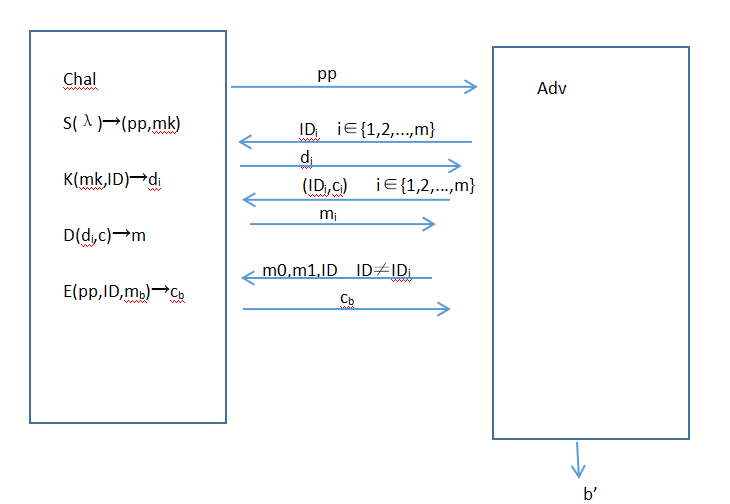
\includegraphics[width=0.5\textwidth]{./figure/CCA} %插入图片,[]中设置图片大小,{}中是图片文件名
		
		\label{e} %用于文内引用的标签

\end{figure}
\centering
$\operatorname{Adv} \varepsilon, \mathcal{A}(k)=\left|\operatorname{Pr}\left[b=b^{\prime}\right]-\frac{1}{2}\right|$
\end{frame}

%------------------------------------------------

\begin{frame}
\frametitle{CPA Security}
Definition 2.2. We say that the IBE system E is semantically secure if for any polynomial time IND-ID-CPA adversary A the function AdvE,A(k) is negligible. As shorthand, we say that E is IND-ID-CPA secure.
\begin{figure}[H]
		\centering %图片居中
		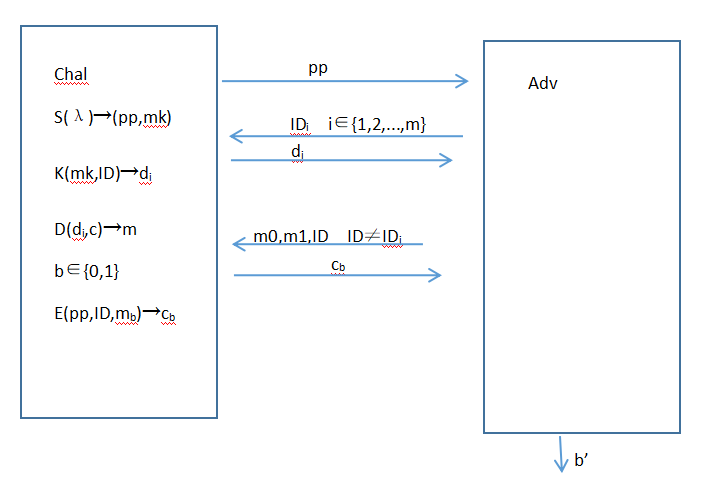
\includegraphics[width=0.5\textwidth]{./figure/CPA} %插入图片,[]中设置图片大小,{}中是图片文件名
		
		\label{e1} %用于文内引用的标签

\end{figure}
\centering
$\operatorname{Adv} \varepsilon, \mathcal{A}(k)=\left|\operatorname{Pr}\left[b=b^{\prime}\right]-\frac{1}{2}\right|$
\end{frame}

%------------------------------------------------

\begin{frame}
\frametitle{Bilinear maps and the Bilinear Diffie-Hellman
Assumption}
Let $ \mathbb{G}_{1}$ and $ \mathbb{G}_{2}$  be two groups of order q for some large prime q. Our IBE system makes use of a bilinear
map$\hat{e}: \mathbb{G}_{1} \times \mathbb{G}_{1} \rightarrow \mathbb{G}_{2}$ between these two groups. The map must satisfy the following properties:\\
\begin{enumerate}
\item Bilinear
\item Non-degenerate
\item Computable
\end{enumerate}
Decision Diffie-Hellman is Easy: The Decision Diffie-Hellman problem (DDH)  in $\mathbb{G}_{1} $ is to distinguish between the distributions $\langle P, a P, b P, a ∂∂∂b P\rangle$ and $\langle P, a P, b P, c P\rangle$ where a, b, c are random in $\mathbb{Z}_{q}^{*}$ and P is random in $\mathbb{G}_{1}^{*}$. Joux and Nguyen  point out that DDH in $\mathbb{G}_{1} $ is easy. To see this, observe that given P, aP, bP, cP $\in \mathbb{G}_{1}^{*}$ we have\\
\centering $c=a b \bmod q \quad \Longleftrightarrow \quad \hat{e}(P, c P)=\hat{e}(a P, b P)$
\end{frame}

\begin{frame}
	\frametitle{CCA secure IBE}
	\begin{figure}[]
		\centering
		\caption{FullIdent Schema}
		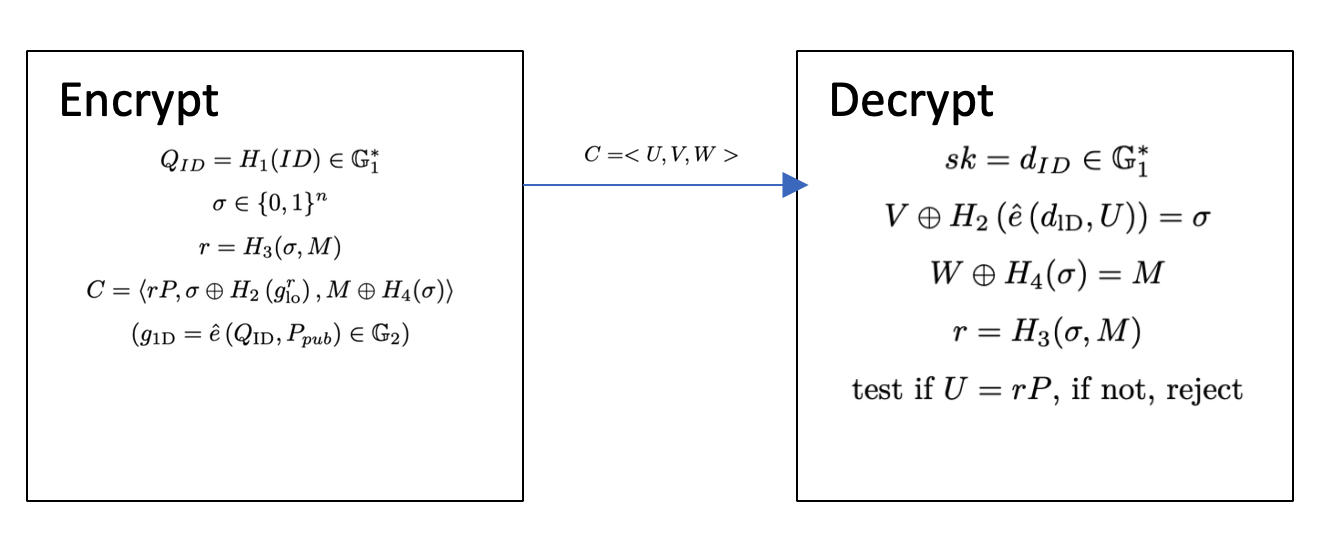
\includegraphics[width=0.7\textwidth]{figure/FullIdent.png}
		\label{}
	\end{figure}
FullIdent is a chosen cipher text secure IBE (IND-ID-CCA), under the assumption of hard BDH. \cite{barreto2002efficient,boneh1998decision}
$$A d v_{\mathcal{G}, \mathcal{B}}(k) \geq 2 F O_{a d v}\left(\frac{\epsilon(k)}{e\left(1+q_{E}+q_{D}\right)}, q_{H_{4}}, q_{H_{3}}, q_{D}\right) / q_{H_{2}}$$ 
\end{frame}

\begin{frame} 
	\frametitle{Relaxing the hashing requirements}
		\begin{figure}[]
			\centering
			\caption{Modified FullIdent}
			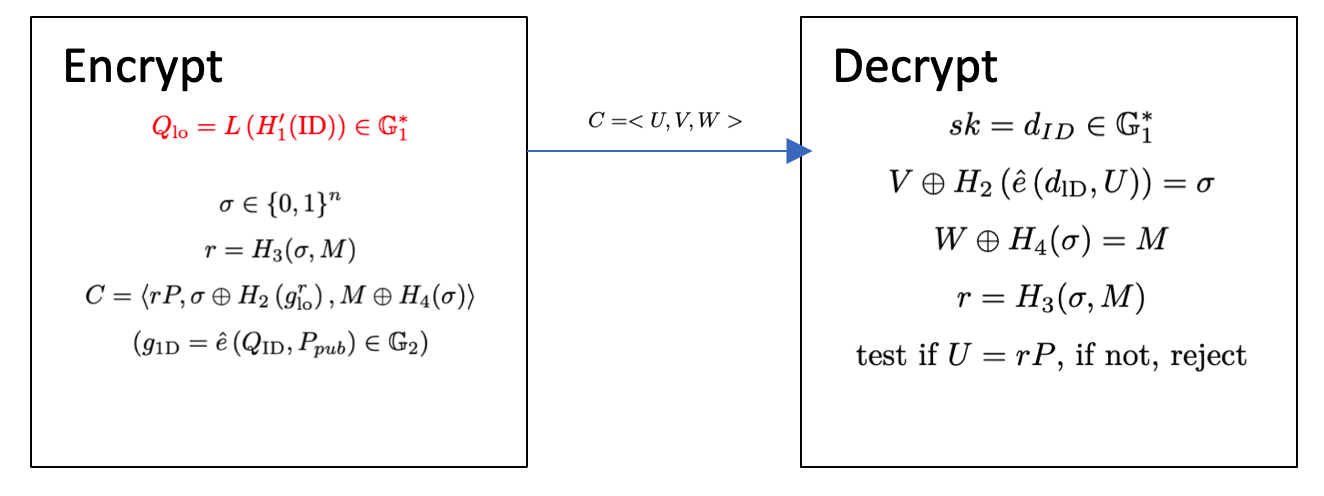
\includegraphics[width=0.7\textwidth]{figure/FullIdent2.png}
			\label{}
		\end{figure}
	Using a deterministic encoding function to map $\mathcal{A}$ onto $\mathbb{G}_1^*$. This modified FullIdent is IND-ID-CCA secure. \cite{boneh2001short}
\end{frame}


% \begin{frame}[fragile] % Need to use the fragile option when verbatim is used in the slide
% \frametitle{Citation}
% An example of the \verb|\cite| command to cite within the presentation:\\~

% This statement requires citation \cite{p1}.
% \end{frame}

%------------------------------------------------

\begin{frame}
\frametitle{References}
\footnotesize{
\begin{thebibliography}{99} % Beamer does not support BibTeX so references must be inserted manually as below
\bibitem[Smith, 2012]{p1} John Smith (2012)
\newblock Title of the publication
\newblock \emph{Journal Name} 12(3), 45 -- 678.


\bibitem{barreto2002efficient}
Paulo~SLM Barreto, Hae~Y Kim, Ben Lynn, and Michael Scott.
\newblock Efficient algorithms for pairing-based cryptosystems.
\newblock In {\em Annual international cryptology conference}, pages 354--369.
  Springer, 2002.

\bibitem{bellare1993random}
Mihir Bellare and Phillip Rogaway.
\newblock Random oracles are practical: A paradigm for designing efficient
  protocols.
\newblock In {\em Proceedings of the 1st ACM conference on Computer and
  communications security}, pages 62--73. ACM, 1993.

\bibitem{boneh1998decision}
Dan Boneh.
\newblock The decision diffie-hellman problem.
\newblock In {\em International Algorithmic Number Theory Symposium}, pages
  48--63. Springer, 1998.

\bibitem{boneh2001identity}
Dan Boneh and Matt Franklin.
\newblock Identity-based encryption from the weil pairing.
\newblock In {\em Annual international cryptology conference}, pages 213--229.
  Springer, 2001.

\bibitem{boneh2001short}
Dan Boneh, Ben Lynn, and Hovav Shacham.
\newblock Short signatures from the weil pairing.
\newblock In {\em International Conference on the Theory and Application of
  Cryptology and Information Security}, pages 514--532. Springer, 2001.

\end{thebibliography}
}
\end{frame}

%------------------------------------------------

\begin{frame}
\Huge{\centerline{The End}}
\end{frame}

%----------------------------------------------------------------------------------------

\end{document} 